\section{Theory}
	A device that translates a continuous physical quantity (typically voltage) to a digital number that indicates the quantity's amplitude is known as an analog-to-digital converter (ADC). A DAC, on the other hand, accepts a binary number and generates an analog voltage or current signal. They are frequently employed in digital systems in conjunction to offer a comprehensive interface with analog devices and output devices for control systems.
	\subsection{Digital to Analog converter (DAC)}
		A Digital to Analog Converter (DAC) has several binary inputs and one output. In general, a DAC's number of binary inputs will be a power of two. DACs are classified into two types: weighted resistor DACs and R/2R ladder DACs. The addition of digital inputs (0 or 1, where 1 equates to 5 volts) in a weighted resistor produces analogue output, which can be added with varied weights depending on their position in the binary number. However, because of the large number of bits, this form of circuit needs a large number of precise resistors. Using an R-2R ladder network in the inverting adder circuit, the R-2R Ladder DAC overcomes this disadvantage and delivers an analogue output that is almost identical to the digital (binary) input. The performance of DAC is characterized by the following:
		\begin{itemize}
			\item \textbf{Resolution:} The resolution of a DAC is determined by the number of bits (N). The resolution is the lowest output increment that the DAC can produce. The resolution of an 8-bit DAC is 8 bits, or one part in $2^8$. This yields a percentage of $0.39\%$.
			\item \textbf{Linearity/ Linear Errors:} The maximum permitted variation from an ideal straight line drawn between the zero-scale and full-scale outputs is defined as linearity. It is frequently expressed as a percentage or as a fraction of an LSB. For an 8-bit DAC, ($\frac{1}{2}$) LSB linearity equates to $0.195\%$.
			\item \textbf{Monotonicity:} If each digital code increase generates an output equal to or greater than the preceding code, the DAC is monotonic. A DAC is often anticipated to be monotonic to increments as tiny as an LSB, but its monotonicity is determined by the smallest increment for which the DAC stays monotonic.
			\item \textbf{Settling time:} The settling time is calculated as the time it takes from the instant a digital input code changes to the time the analogue output achieves its matching new value within a given error band. Typically, the output is anticipated to settle within a $\frac{1}{2}$ LSB error range. Typically, the worst-case settling time is evaluated between the zero-scale and full-scale codes.
			\item \textbf{Accuracy:} The maximum divergence between the actual converter output and the ideal converter output is defined as absolute accuracy. The greatest variation after removing gain and offset errors is referred to as relative accuracy.
		\end{itemize}

	\subsection{Analog to Digital Converter}
		\begin{figure}[H]
			\centering
			\label{theory:1}
			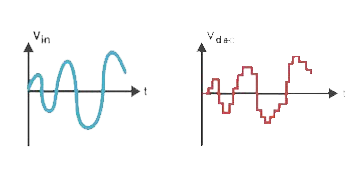
\includegraphics[width=0.6\columnwidth]{images/theory1.png}
			\caption{Analog to Digital Converter}
		\end{figure}

		It can be done in many different ways to take an analog voltage signal and convert it into an equivalent digital signal. While many analog-to-digital converter chips are available, it is possible to build a simple ADC using discrete components.

		One simple and easy way is by using parallel encoding, also known as flash, simultaneous, or multiple comparator converters, in which comparators are used to detect different voltage levels and output their switching state to an encoder.
